% Created 2023-10-01 Sun 21:40
% Intended LaTeX compiler: pdflatex
\documentclass[11pt]{article}
\usepackage[utf8]{inputenc}
\usepackage[T1]{fontenc}
\usepackage{graphicx}
\usepackage{longtable}
\usepackage{wrapfig}
\usepackage{rotating}
\usepackage[normalem]{ulem}
\usepackage{amsmath}
\usepackage{amssymb}
\usepackage{capt-of}
\usepackage{hyperref}
\author{Yusheng Zhao}
\date{\textit{<2023-10-01 Sun>}}
\title{Homework 1}
\hypersetup{
 pdfauthor={Yusheng Zhao},
 pdftitle={Homework 1},
 pdfkeywords={},
 pdfsubject={},
 pdfcreator={Emacs 29.1 (Org mode 9.7)}, 
 pdflang={English}}
\begin{document}

\maketitle
\section{Answer 2}
\label{sec:org543eb0e}
In this problem, I will investigate the influence of number of epochs a two
layer neural is trained on the accuracy of the model. I investigate for five different types of functions.
\subsection{Smooth vs Non-smooth function}
\label{sec:org73c551b}
For the smooth function, I use the function \(f(x) = x\), and for the
non-smooth function, I use the function \(f(x) = x - \lfloor x \rfloor\).

As indicated in the graph below, the non-smooth is more difficult to train than
the smooth function. I.e, it reaches low loss in later epochs. The accuracy of
the model for the non-smooth function also starts out to be worse than that of
the smooth function.

\begin{center}
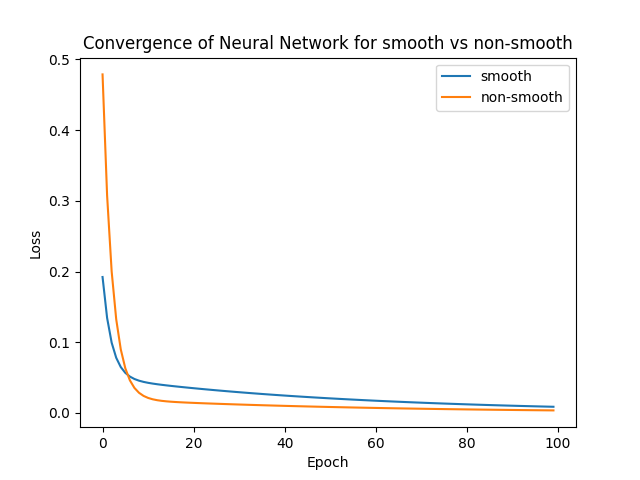
\includegraphics[width=.9\linewidth]{plots/convergence_smooth vs non-smooth.png}
\end{center}
\end{document}